\begin{figure}[!htb]
\begin{center}
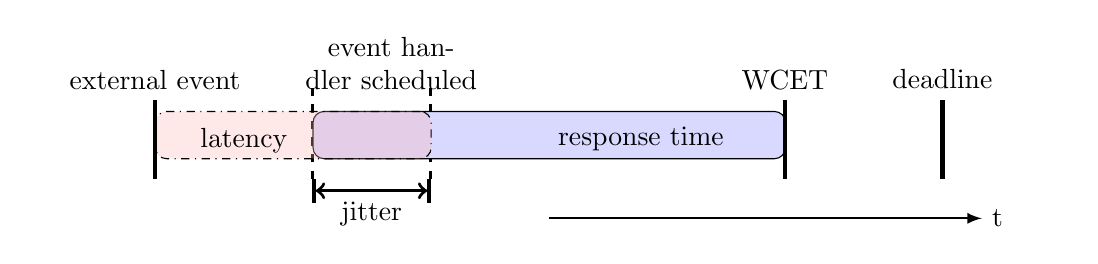
\begin{tikzpicture}
%\draw[gray, very thick, solid, >-<]  (0,1.5) -- (9,1.5) node at (4,1.5) [above] {relative deadline};
%\draw[black, very thick, ->]  (0,0) -- (10,0) node at (11,0) {time};
\draw[black, very thick, dashed] (2.0,0) -- (2.0,1.25) node at (3,1) [text width=3cm, above, align=center] {event handler scheduled};
\draw[black, very thick, dashed] (3.5,0) -- (3.5,1.25);

\node at (2.0,0.25)[rectangle, draw=black, fill=blue!15, rounded corners, minimum height = 0.6cm, minimum width = 6cm, anchor=south west] (resptime) {};

\begin{scope}[fill opacity=0.3]
\node at (0,0.25)[rectangle, draw=black, dashdotted, fill=red!30, rounded corners, minimum height = 0.6cm, minimum width = 3.50cm, anchor=south west] (latency) {};
%\node at (2.0,0.25)[rectangle, draw=black, postaction={pattern=north east lines}, minimum height = 0.6cm, minimum width = 1.5cm, anchor=south west] (overlap) {};
\end{scope}

\node [above left, inner sep=2pt] at (latency.south) {latency};
\node [above right, inner sep=3pt] at (resptime.south) {response time};

\draw[black, very thick, solid] (0,0) -- (0,1) node at (0,1) [text width=3cm, above, align=center] {external event};
\draw[black, very thick, solid] (8,0) -- (8,1) node at (8,1) [text width=3cm, above, align=center] {WCET};
\draw[black, ultra thick, solid] (10,0) -- (10,1) node at (10,1) [text width=3cm, above, align=center] {deadline};

\draw[black, very thick, solid, |<->|] (2.0,-0.15) -- (3.5,-0.15) node (jitter) at (2.75,-0.15) [below] {jitter};

%\node (latlabel) at (1,-1.0) {latency};
%\node (jitlabel) at (4,-1.0) {jitter};
%\node (rtlabel) at (8,-1.0) {response time};

\begin{scope}[>=latex]
	%\draw [thick, ->] (latlabel) to [bend right=45] (latency.center);
	%\draw [thick, ->] (rtlabel) to [bend left=45] (resptime.center);
    	%\draw [thick, ->] (jitlabel) to [bend left=45] (jitter.center);
	\draw[black, thick, ->] (5,-0.5) -- (10.5,-0.5) node [right] {t};
\end{scope}
\end{tikzpicture}
\end{center}
\ifreport
\caption{Real-time task interrupt latency and jitter}
\fi
\label{fig-latency-jitter}
\end{figure}
